% Session 8 -- the emergent gauge structure: link phases are gauge-dependent, plaquette
% Placement: sec. "Emergent gauge symmetry and vison excitations", after the square-lattice
% example.
% Rendered by figures/blender/s08f05_gauge_vison.py, labels in figures/overlays/s08f05_gauge_vison.tex.
\begin{aqmfigure}{fig:s08:gauge}{The emergent gauge theory of the parton construction, and its
excitation, seen from above. (a) The mean-field bond variable is defined on the links,
$\chi_{ij}=|\chi_{ij}|e^{i\theta_{ij}}$, drawn as a dial at the phase $\theta_{ij}$, and the local
phase rotation (8.16) on one site shifts every link phase by $\theta_i-\theta_j$, which changes the
two red needles. When we go once around a plaquette, each site phase appears twice with opposite
signs, so the flux $\Phi=\prod e^{i\theta_{ij}}$ does not change. The link variables are pure gauge,
and the flux is physical. This is the reason why two mean-field solutions related by (8.16) describe
the same spin liquid. (b) As a result, the flux is what labels the state. With $\Phi=+1$ on every
plaquette as the ground state, flipping a single plaquette to $\Phi=-1$ costs energy, and no gauge
transformation can remove it. This localized defect of the gauge field is a \textbf{vison}. Which
links have the minus sign is a gauge choice, here a string from the edge, and it can be moved
freely, while the shaded plaquette cannot be moved.}
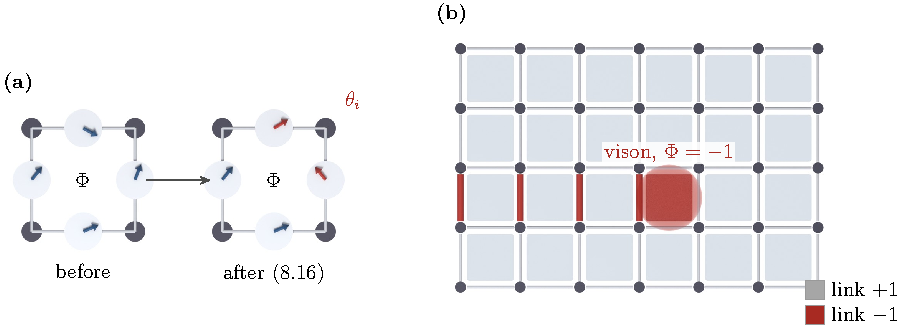
\includegraphics{figures/pdf/s08f05_gauge_vison.pdf}
\end{aqmfigure}
